%
% This is the LaTeX template file for lecture notes for CS294-8,
% Computational Biology for Computer Scientists.  When preparing 
% LaTeX notes for this class, please use this template.
%
% To familiarize yourself with this template, the body contains
% some examples of its use.  Look them over.  Then you can
% run LaTeX on this file.  After you have LaTeXed this file then
% you can look over the result either by printing it out with
% dvips or using xdvi.
%
% This template is based on the template for Prof. Sinclair's CS 270.

\documentclass[twoside]{article}
\usepackage{mathtools}
\usepackage{graphicx}
\usepackage[pdftex]{pict2e}
\usepackage{varwidth}
\usepackage{amsmath}
\usepackage{amssymb}
\usepackage{graphics}
\usepackage{dsfont}
\setlength{\oddsidemargin}{0.25 in}
\setlength{\evensidemargin}{-0.25 in}
\setlength{\topmargin}{-0.6 in}
\setlength{\textwidth}{6.5 in}
\setlength{\textheight}{8.5 in}
\setlength{\headsep}{0.75 in}
\setlength{\parindent}{0 in}
\setlength{\parskip}{0.1 in}

%
% The following commands set up the lecnum (lecture number)
% counter and make various numbering schemes work relative
% to the lecture number.
%
\newcounter{lecnum}
\renewcommand{\thepage}{\thelecnum-\arabic{page}}
\renewcommand{\thesection}{\thelecnum.\arabic{section}}
\renewcommand{\theequation}{\thelecnum.\arabic{equation}}
\renewcommand{\thefigure}{\thelecnum.\arabic{figure}}
\renewcommand{\thetable}{\thelecnum.\arabic{table}}

%
% The following macro is used to generate the header.
%
\newcommand{\lecture}[4]{
   \pagestyle{myheadings}
   \thispagestyle{plain}
   \newpage
   \setcounter{lecnum}{#1}
   \setcounter{page}{1}
   \noindent
   \begin{center}
   \framebox{
      \vbox{\vspace{2mm}
    \hbox to 6.28in { {\bf Optimization Algorithms
                        \hfill Winter 2023} }
       \vspace{4mm}
       \hbox to 6.28in { {\Large \hfill Lecture #1: #2  \hfill} }
       \vspace{2mm}
       \hbox to 6.28in { {\it Lecturer: #3 \hfill Scribes: #4} }
      \vspace{2mm}}
   }
   \end{center}
   \markboth{Lecture #1: #2}{Lecture #1: #2}
   {\bf Note}: {\it LaTeX template courtesy of UC Berkeley EECS dept.}

   {\bf Disclaimer}: {\it These notes are based on the freely available online lectures by Constantine Caramanis.
}
   \vspace*{4mm}
}

%
% Convention for citations is authors' initials followed by the year.
% For example, to cite a paper by Leighton and Maggs you would type
% \cite{LM89}, and to cite a paper by Strassen you would type \cite{S69}.
% (To avoid bibliography problems, for now we redefine the \cite command.)
% Also commands that create a suitable format for the reference list.
\renewcommand{\cite}[1]{[#1]}
\def\beginrefs{\begin{list}%
        {[\arabic{equation}]}{\usecounter{equation}
         \setlength{\leftmargin}{2.0truecm}\setlength{\labelsep}{0.4truecm}%
         \setlength{\labelwidth}{1.6truecm}}}
\def\endrefs{\end{list}}
\def\bibentry#1{\item[\hbox{[#1]}]}

%Use this command for a figure; it puts a figure in wherever you want it.
%usage: \fig{NUMBER}{SPACE-IN-INCHES}{CAPTION}
\newcommand{\fig}[3]{
			\vspace{#2}
			\begin{center}
			Figure \thelecnum.#1:~#3
			\end{center}
	}

 
% Use these for theorems, lemmas, proofs, etc.
\newtheorem{theorem}{Theorem}[lecnum]
\newtheorem{lemma}[theorem]{Lemma}
\newtheorem{proposition}[theorem]{Proposition}
\newtheorem{claim}[theorem]{Claim}
\newtheorem{corollary}[theorem]{Corollary}
\newtheorem{definition}[theorem]{Definition}
\newenvironment{proof}{{\bf Proof:}}{\hfill\rule{2mm}{2mm}}

% **** IF YOU WANT TO DEFINE ADDITIONAL MACROS FOR YOURSELF, PUT THEM HERE:

\begin{document}

%FILL IN THE RIGHT INFO.
%\lecture{**LECTURE-NUMBER**}{**DATE**}{**LECTURER**}{**SCRIBE**}
\lecture{4}{Dimension-free convex optimization
}{Constantine Caramanis}{Chanho Jung}
%\footnotetext{These notes are partially based on those of Nigel Mansell.}

% **** YOUR NOTES GO HERE:

% Some general latex examples and examples making use of the
% macros follow.  
%**** IN GENERAL, BE BRIEF. LONG SCRIBE NOTES, NO MATTER HOW WELL WRITTEN,
%**** ARE NEVER READ BY ANYBODY.

\section{Oracle Lower Bounds}

A natural question now that we've derived this is are these optimal. so is it possible for example that our analysis was loose or is it impossible that there is a better algorithm out there. this is by itself a subtle question to ask because there's no such thing as an optimal algorithm for a specific optimization problem. every specific optimization algorithm problem has an answer so the algorithm that just outputs that answer is unbeatable for that specific function but of course is not going to be very good for other functions. so this is how we're gonna make this concept a little bit more precise and this will allow us to reason about optimality of certain algorithms. 

\subsection{Review: Rates of Convergence - are the optimal?}

\textbf{Subgradient method} : $x_{t+1} = x_t- \eta g_t$, where $g_t \in \partial f(x_t)$

\textbf{Gradient method} : $x_{t+1} = x_t- {\eta}{\nabla}f(x_t)$

\textbf{Subgradient method for Lipschitz convex functions} : Lipschitz means that subgradients are uniformly bounded so ${\exists}$${G}$, $||g||_2$ ${\leq}$ $G$, ${\forall}g$ ${\in}$ $\partial$$f(x)$, as long as $f$ is convex and satisfies this property then we saw that the sub gradient method guarantees that after T iterations, $$ Error: \mathcal{O}\left({1 \over {\sqrt{T}}}\right)  \leftrightarrow \mathcal{O}\left({1 \over \epsilon^2}\right) $$

\textbf{Gradient descent for smooth convex functions} : $$ Error: \mathcal{O}\left({1 \over T}\right)  \leftrightarrow \mathcal{O}\left({1 \over \epsilon}\right) $$

\textbf{Gradient descent for $\beta$-smooth and $\alpha$-strongly convex functions} : $$ Error: \mathcal{O}\left(\left({\kappa-1 \over \kappa+1}\right)^T\right)  \leftrightarrow \mathcal{O}\left(\kappa{\log\left({1 \over \epsilon}\right)}\right) , \kappa = {\beta \over \alpha}  $$



\subsection{Oracle model of computation}

% \begin{math}
% \end{math}
\textbf{What do we know about our functions?} : $$min:f(x)
, st: x \in \mathfrak{X}=\mathds{R}^d$$

the way to make precise this idea of complexity and optimality in terms of how of convergence rate is to say what do we know about our function what do we use for every single algorithm that we've seen so far we found that all we need is to be able to evaluate the function and also evaluate its gradient or to get an arbitary element of the sub differential. in other words think about this as though we don't actually know our function $f$ at all. all we have access to is something that I'll call an Oracle. 


$$x\longrightarrow
\fbox{\begin{varwidth}{\dimexpr\textwidth-2\fboxsep-2\fboxrule\relax}
First order Oracle

\end{varwidth}}
\longrightarrow f(x),{\nabla}f(x) {\text{ or }} g_x {\in} {\partial}f(x)$$	 


Let's consider only algorithms that can be cast as having access to our function only through this Oracle.
Suppose the only access we have to our function $f$ is through the Oracle. then we can frame the question as follows.
$$\text{How many calls to the Oracle do we need in the worst case over a class of functions, in order to guarantee error }\epsilon?$$

we're making no assumptions about what you do once you get back the gradient or the subgradient of $f$. you could be doing some incredibly complicated procedure possibly exponential time. This question doesn't care about that it's just saying how many times you need to evaluate this Oracle.

\subsection{Oracle based lower bounds}

\textbf{For the class of Lipchitz convex functions} : the subgradient method is unimprovable, so it is optimal.

this is the class for which subgradient method guarantees $\mathcal{O}\left({1 \over {\sqrt{T}}}\right)$, there is no algorithm which can guarantee error better than $\mathcal{O}\left({1 \over {\sqrt{T}}}\right)$ for all functions in this class(In the worst case)

{\bf Note}: {\it That doesn't mean if I have a particular Lipschitz and convex function I can't find a better algorithm than subgradient descent. It means that I can't find an algorithm that uses fewer than T square root evaluations.If you don't have any other information about your function then this is the best.}

\textbf{For the case of smooth functions} : can be imporved
\begin{center}
the lower bound is $\mathcal{O}\left({1 \over T^2}\right) \leftrightarrow \mathcal{O}\left({1 \over \sqrt{\epsilon}}\right)$
\end{center}

\textbf{For $\beta$-smooth and $\alpha$-strongly convex functions} : can be imporved
$$ \text{the lower bound is  } \mathcal{O}\left(\left({\sqrt{\kappa}-1 \over \sqrt{\kappa}+1}\right)^T\right)  \leftrightarrow \mathcal{O}\left(\kappa{\log\left({1 \over \epsilon}\right)}\right) , \kappa = {\beta \over \alpha}{\geq}{ 1 }\Rightarrow{\sqrt{\kappa}}{<}{\kappa}  $$

\subsection{Discussion about the oracle model}

\textbf{Is the assumption reasonable? What is the takeaway?} : If we develop any algorithm that only uses evaluations of $f(x)$ and $\nabla{f(x)}$, then we are bound by the Oracle lower bound

this is the only thing we know about our function. 
$$x\longrightarrow
\fbox{\begin{varwidth}{\dimexpr\textwidth-2\fboxsep-2\fboxrule\relax}
First order Oracle

\end{varwidth}}
\longrightarrow f(x),{\nabla}f(x) {\text{ or }} g_x {\in} {\partial}f(x)$$

it' very rare that this is in fact the model that we have. In that sense, how is this helpful to us well it says the following thing one way to think about this Oracle model and what the takeaway is or what it word guarantees is if we develop any algorithm that only uses evaluations of $f(x)$ and $\nabla{f(x)}$.then we can imagine that we have only access to the Oracle in other words even if you know $f$ if what you're the algorithm that you develop only uses evaluations of $f$ and $\nabla{f(x)}$. then even if you didn't know $f$ and you only knew you only had access to the Oracle you would be running exactly the same algorithm and therefore that means that you're bound by whatever lower bounds we have from the Oracle model. 

\section{Accelerated Gradient Descent}

we're now going to talk about an improved algorithm that uses gradients and point evaluations of function in the case where our function has smoothness. 

% \textbf{Recall} $f$ is $\beta$-smooth,gradient descent was able to guarantee a convergence rate of $\mathcal{O}\left({1 \over T}\right)$.But the lower bound gave something better $\mathcal{O}\left({1 \over T^2}\right)$

\textbf{Recall} 

$f$ is $\beta$-smooth, GD: $\mathcal{O}\left({1 \over T}\right), $LB: $\mathcal{O}\left({1 \over T^2}\right)$

$f$ is $\beta$-smooth and $\alpha$-strongly convex, GD: $\mathcal{O}\left(\left({\kappa-1 \over \kappa+1}\right)^T\right)$, LB: $\mathcal{O}\left(\left({\sqrt{\kappa}-1 \over \sqrt{\kappa}+1}\right)^T\right)$
, $\kappa = {\beta \over \alpha}$

so, we want to see if we can do better
\subsection{Accelerated Gradient Descent: momentum}

The key idea here is a concept called momentum. so let's recall what the basic gradient descent algorithm

\textbf{Gradient method} : $x_{t+1}$ = $x_t$- ${\eta}$${\nabla}$$f(x_t)$

the idea of momentum is to include a term here that capture some aspect of where I was before the direction that I was moving in.so the name is suggestive.


\textbf{Idea of momentum} : $x_{t}$ - $x_{t-1}$

$x_{t}$ - $x_{t-1}$ gives me the direction in which I was moving in before.
\begin{center}
    

\setlength{\unitlength}{1cm}
\begin{picture}(4,4)      % picture box will be 6cm wide by 6cm tall
  \put(0,0){\vector(2,1){4}}{\makebox(-0.5,0){$x_t$}}  % for every 2 over this vector goes 1 up
    \put(2,1){\makebox(-2,0){- ${\eta}$${\nabla}$$f(x_t)$}}
  \put(4,2){\vector(1,-1){2}}
    \put(5,4){\makebox(-2,-5){$x_{t+1}$}}  
  \put(4,2){{\vector(1,0.5){2}}}
    \put(3,3){\makebox(2,0)[l]{momentum}}
  \put(6,3){\vector(1,-1){2}}
    \put(3,3){\makebox(4,-4)[r]{- ${\eta}$${\nabla}$$f(x_{t+1})$}}
  \put(6,-0.2){\makebox(0,0){$x_{t+2}$}}
\end{picture}

\end{center}
\subsection{Acceleration: Smooth and strongly convex functions}

the algorithm sometimes called momentum sometimes called accelerated gradient descent is a following.
\begin{center}
$min$: $f(x)$ , $f$ is $\beta$-smooth and $\alpha$-strongly convex

Gradient descent: $x_{t+1}$ = $x_t$- ${\eta}$${\nabla}$$f(x_t)$ , ${\eta}$=${1 \over \beta}$

Accelerated Gradient descent(momentum): initialize: $x_1$ = $y_1$ = $x_{init}$, after t iterations

 $y_{t+1}$ = $x_t$ - $\eta$$\nabla{f(x_t)}$
 
 $x_{t+1}$ = ${\left(1+{\sqrt{\kappa}-1 \over \sqrt{\kappa}+1}\right)}y_{t+1}$ - ${\left({\sqrt{\kappa}-1 \over \sqrt{\kappa}+1}\right)}y_{t}$ 

\end{center}

 $x_{t+1}$ is convex combination between $y_{t+1}$ and $y_t$. $x_{t+1}$ depends not only on $x_t$ but also $x_{t-1}$. because $y_{t+1}$ is a function of $x_{t}$ and therefore $y_{t}$ is a function of $x_{t-1}$. So $x_{t+1}$ is a function of the past two iterates. that's exactly where the momentum comes in.

 {\bf Theorem}: {\it $f(y_t)$ - $f(x^*)$ $\leq$ ${\alpha+\beta \over 2}$$||x_1-x^*||^2$$\cdot{exp(-{(t+1)\over{\sqrt{\kappa}}})}$}

 we have improved from $\kappa \rightarrow \sqrt{\kappa}$.
\subsection{Acceleration vs Gradient descent: an example}

\begin{figure}[h] %%% t: top, b: bottom, h: here
\begin{center}
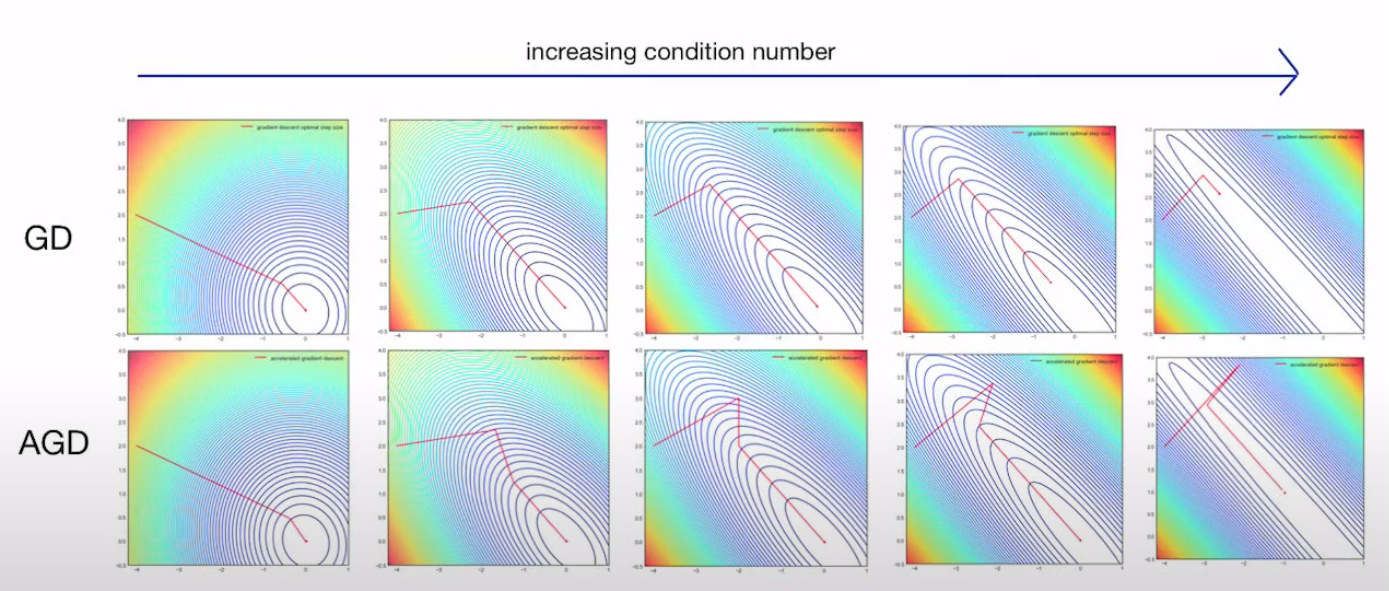
\includegraphics[width=1.0\linewidth]{fig1.png}
\end{center}
\caption{Trajectories of GD and AGD for different values of $\kappa$ = $\beta \over \alpha$}
\label{fig:long}
\label{fig:onecol}

\end{figure}

$\beta$ as we've seen is equal to the largest eigenvalue and $\alpha$ is equal to the smallest eigenvalue. this is why where this terminology comes in of the condition number as a standart definition in this case of the condition number of a matrix. 

Let's look at what we have starting from small condition number. small condition number means that the largest eigenvalue and smallest eigenvalue are pretty close together. contours are very close to being spherical which is what we would expect if the condition number is close to one. 

gradient descent is doing what is locally best ignoring everything else it's just looking very locally and doing the moving in the optimal direction infinitesimally optimal direction. as a condition number increase here the trajectories of GD and AGD begin to look significantly different.{\it we're starting to see the impact of momentum.} the third column or it's even more pronounced in the fourth and fifth column you can see that in the same number of iterations and they both run for their optimal step size which is $1 \over \beta$, AGD is outperforming GD. 

we see two things. first of all AGD is significantly outperforming GD but also we start seeing increasingly pronounced overshoot which is something else that we would expect from having this momentum terms.

\textbf{Conclusion}
GD is always moving to a closer and closer contour.GD is in fact a descent algorithm it strictly improves at every single iteration untill it gets to the optimal solution but this is again not the case for AGD. There are situations where AGD takes a step and it actually will increase the function value nevertheless it is faster and it achieves the lower bounds so in that sense it's optimal.

\subsection{Acceleration: smooth functions}
We will show we match $LB: \mathcal{O}\left({1 \over T^2}\right)$ compared to convergence rate :$\mathcal{O}\left({1 \over T}\right)$
\begin{center}

$f$ is convex and $\beta$-smooth

Gradient step: $x^{+}$ = $x$ - ${\eta}$${\nabla}$$f(x_t)$ , ${\eta}$=${1 \over \beta}$

Momentum term: $d_t$ = $\gamma_t{\left(x_t - x_{t-1}\right)}$ , $\gamma_t$ is a parameter we choose

GD algorithm: $x_{t+1}$ = $(x_t)^+$

Nesterov Acceleration: $(x_t + d_t)^+$ = $x_t+d_t$ - $\eta \nabla f(x_t+d_t)$
\end{center}

\textbf{Proof of convergence rate}

Thinking back to our proof of $\mathcal{O}\left({1 \over T}\right)$ convergence rate for a gradient descent there were two things that we needed repeatedly namely upper and lower bounds on $f$.

$f$ is convex : $f(x) - f(y) \leq \langle\ \nabla f(x), x-y\rangle$. this is a linear lower bound on $f(y)$. And because of smoothness I also have a quadratic upper bound on $f(y)$. if we phrase if we write $y$ as the update.

$f(y) \leq f(x) + \langle\ \nabla f(x), x-y\rangle + {\beta \over 2}{||y-x||}^2$. 

$f$ is $\beta$-smooth : $f(x^+) - f(x) \leq - {1\over {2\beta}} ||\nabla f(x)||^2$, $\eta = {1 \over \beta}$ . we've mentioned over and over again this is a statement that gradient descent is in fact a descent algorithm and this was the basis the starting point for the proof.

Notation: $\delta_t = f(x_t) - f(x^*) \geq 0$ , $g_t = -{1 \over \beta}\nabla f(x_t+d_t)$ : $x_{t+1} = x_t +d_t+g_t$

there is two quantities that I want to bound.

(a) $\delta_{t+1} - \delta_{t} \leq -{\beta \over 2}{\left(||g_t||^2 + 2g_t^Td_t\right)}$

(b) $\delta_{t+1} \leq -{\beta \over 2}{\left(||g_t||^2 + 2g_t^T\left(x_t+d_t-x^*\right)\right)}$
\begin{center}

\begin{align*}
\delta_{t+1} - \delta_{t} &\leq -{\beta \over 2}{\left(||g_t||^2 + 2g_t^Td_t\right)} \\
&=  -{\beta \over 2}{\left({1 \over \beta^2}{||\nabla f(x_t+d_t)||}^2 -{2 \over \beta}\nabla f(x_t+d_t)^Td_t\right)} \\
&= -{2 \over \beta}||\nabla f(x_t+d_t)||^2+\nabla f(x_t+d_t)^Td_t \\
&\geq f \left(x_t+d_t-\eta \nabla f(x_t+d_t)\right) -f(x_t+d_t)+f(x_t+d_t) -f(x_t) \leftarrow \text{This is LHS of (a)}\\
\end{align*}
\end{center}


\begin{center}

$(\lambda_t - 1)\cdot(a) + 1\cdot(b) \leq -{\beta \over 2}\left[{1 \over \lambda_t}\left(||x_t+\lambda_t d_t-x^*+\lambda_t g_t||^2-||x_t+\lambda_t d_t - x^*||^2\right)\right]$

we would like for the RHS to be telescoping. 

we want, $x_t+\lambda_t d_t - x^*+\lambda_t g_t$ = $x_{t+1}+\lambda_{t+1}d_{t+1}-x^*$

recall : $d_{t+1} = \gamma_{t+1}(d_t+g_t)$

\begin{align*}
x_t+\lambda_t d_t - x^*+\lambda_t g_t &= x_{t+1}+\lambda_{t+1}d_{t+1}-x^*\\
&=x_t+d_t+g_t+\lambda_{t+1}\gamma_{t+1}(d_t+g_t)-x^*
\end{align*}

if $\lambda_t(d_t+g_t) = (\lambda_{t+1}\gamma_{t+1}+1)(d_t+g_t)$ , then we can get what we want.

$\gamma_t$ is a parameter that I'm able to choose. so I'm going to choose $\gamma_{t+1}$,$\gamma_t$ to make this telescope.

${2 \over \beta}u_{t+1}$ $\coloneqq ||x_t+\lambda_t d_t-x^*+\lambda_t g_t||^2$, 

${2 \over \beta}u_t$ $\coloneqq ||x_t+\lambda_t d_t - x^*||^2$

multiplying by $\lambda_t$ and remeber $\lambda_t$ is also a free parameter. $\gamma_t$ is a function of $\lambda_t$ that still allow me to pick,

$\lambda_t^2\cdot(\delta_{t+1}) - (\lambda_t^2-\lambda_t)\delta_t$ $\leq u_t - u_{t+1}$

we're going to pick $\lambda_t$ to make this telescope. that is It holds $\lambda_t^2 - \lambda_t=\lambda_{t-1}^2$ : $\lambda_t$ $\approx t$ will satisfy this, specifically: $\lambda_t = {-1\pm\sqrt{1+4\lambda_{t-1}^2} \over 2}$ 

sum both sides for T iterations:

$\lambda_T^2\delta_{T+1}-\lambda_0 \delta_1 \leq u_0 - u_T \leq u_0$ 
 $\Rightarrow{\delta_{T+1}\leq {constant \over \lambda_T^2}}$

 $\Rightarrow f(x_t)-f(x^*) \leq {constant\over T^2}$
\end{center}

\textbf{Summary} : 

1. Lower bounds for smooth,convex optimization are matched by GD+Monentum method.

2. Choose the coefficients carefully.


% \section*{References}
% \beginrefs
% \bibentry{AGM97}{\sc N.~Alon}, {\sc Z.~Galil} and {\sc O.~Margalit},
% On the Exponent of the All Pairs Shortest Path Problem,
% {\it Journal of Computer and System Sciences\/}~{\bf 54} (1997),
% pp.~255--262.

% \bibentry{F76}{\sc M. L. ~Fredman}, New Bounds on the Complexity of the 
% Shortest Path Problem, {\it SIAM Journal on Computing\/}~{\bf 5} (1976), 
% pp.~83-89.
% \endrefs

\nocite{Beck2017,bubeck2015convex,caramanis2020opt,deisenroth2020mathematics}
\bibliography{../../references}
\bibliographystyle{plain}


\end{document}





